\chapter{Исследование масштабируемости модели общей циркуляции океана}\label{ch:inmsom/ch3}

\section{Тестирование Азовского Моря}\label{sec:inmsom/ch3/sec1}

	В этой главе приводятся результаты по тестированию метода нагрузки балансировки вычислений  с использованием кривых Гильберта уже применительно к полной трехмерной сигма-модели циркуляции океана INMOM, которая была описана в главах \ref{ch:inmsom/ch1}, \ref{ch:inmsom/ch2}.
	
	Тестирование модели проводилось на кластере ИВМ РАН. Кластер состоит из головного узла, вспомогательного узла и вычислительных узлов,
	объеденных в разные группы. Тестирование проводилось преимущественно на группе вычислительных узлов x8core, состоящих из двух 8-ядерных процессоров Intel Xeon E5-2665@2.40ГГц
	и с 64 Гб оперативной памяти.
%	Характеристики вычислительных узлов в группе x8core:
%	\begin{itemize}
%	\setlength\itemsep{0.0em}
%	\item Compute Node Arbyte Alkazar+ R2Q50.
%	\item 16 ядер (два 8-ядерных процессора Intel Xeon E5-2665@2.40ГГц).
%	\item Оперативная память: 64 Гб.
%	\end{itemize}
	На кластере установлены последние версии компиляторов Intel Fortran (ifort) и библиотек MPI, с помощью
	которых собиралась и тестировалась модель.
	
	Метод балансировки нагрузки вычислений рассматривался на следующих сетках блоков:
	по 8 блоков на ядро для 128 ядер и по 4 блока на ядро для всех остальных. 
	Тестирование проводилось для акватории Азовского моря, см. \ref{sec:ch3/sec2}. Шаг по времени был выбран равным 30 секундам.
	
%	\begin{tabular}{|l|l|l|l|l|l|l|}
%    \hline
%    Cores    & 1 & 4 & 16 & 64 & 128 & 256 \\ 
%    \hline
%    Uniform  & 1 & 4 & 16 & 64 & 128 & 256 \\ 
%    \hline
%    Hilbert  & 1 & 4 & 16 & 64 & 128 & 256 \\ 
%    \hline
%    METIS    & 1 & 4 & 16 & 64 & 128 & 256 \\ 
%    \hline
%    \end{tabular}
%    }
%    \end{subtable}
%    \end{table}
	
	На рис. \ref{fig:inmom_hilbert1} и рис. \ref{fig:inmom_hilbert2} показано ускорение параллельной версии модели INMOM с методом балансировки, использующим кривые Гильберта,
    в сравнении с равномерным разбиением без балансировки и в сравнении с разбиением,
    полученным с помощью библиотеки METIS.      
    %Ускорение считалось по формуле (\ref{eq:speedup}),
    %где в качестве $T_{init}$ было взято время работы параллельной версии модели на 4 ядрах без балансировки нагрузки вычислений, на рис. \ref{fig:timemodelsteps} показано $T_{init}$ для различных блоков модели. 
    Из графиков видно, что методы балансировки нагрузки вычислений дают 
    сверхлинейное ускорение для расчетов температуры и солености %(шаг 9 в модели, см. главу 4)
    и для
    расчета переноса и диффузии компонентов скорости. % (шаг 10 в модели, см. главу 4). 
    Это связано с тем, что при увеличении числа ядер, 
    большая часть блоков, попадающих полностью на сушу, выпадает из рассмотрения. % (см. таблицу 2).
    Более того, размер каждого блока становится мал и работа с кэш памятью становится наиболее эффективной.
    Исследования масштабируемости показали, что самым узким местом при распараллеливании модели океана является баротропная адаптация. % (шаг 16 в модели, см. главу 4).
    Это связано с тем, что
    на этой стадии решается линейная система алгебраических уравнений.
    Как уже было более подробно описано в \ref{ch:inmsom/ch2}, в качестве основного
    решателя был выбран
    метод GMRES с предобуславливателем ASM из библиотеки PETSc.
    Хоть и для этой стадии модели было получено самое низкое ускорение - 
    все равно видна эффективность метода балансировки нагрузки по сравнению с равномерным
    разбиением без балансировки.
    Для общего расчетного времени модели метод балансировки нагрузки дает почти линейное ускорение и по сравнению с равномерным разбиением без балансировки нагрузки ускорение больше в $\sim 1.7$ раза.
	Из графиков и таблицы \ref{tab:LB} видно, что метод балансировки нагрузки с использованием кривой Гильберта строит разбиения не хуже чем METIS.
	Для 128 и 256 ядер видно даже преимущество в ускорении, полученном с помощью
	этого метода, в сравнении с METIS.
	Похожие результаты были получены и при сравнении методов балансировки нагрузки
	применительно к уравнениям мелкой воды, разрешаемых по явной схеме по времени. % (см. главу 7.2). 
    В общем можно сделать вывод, что метод балансировки нагрузки вычислений с 
    использованием кривой Гильберта - это хорошая альтернатива библиотеке METIS.
    
	\begin{figure}[htb!]
    \begin{minipage}[h]{0.48\linewidth}
    \center{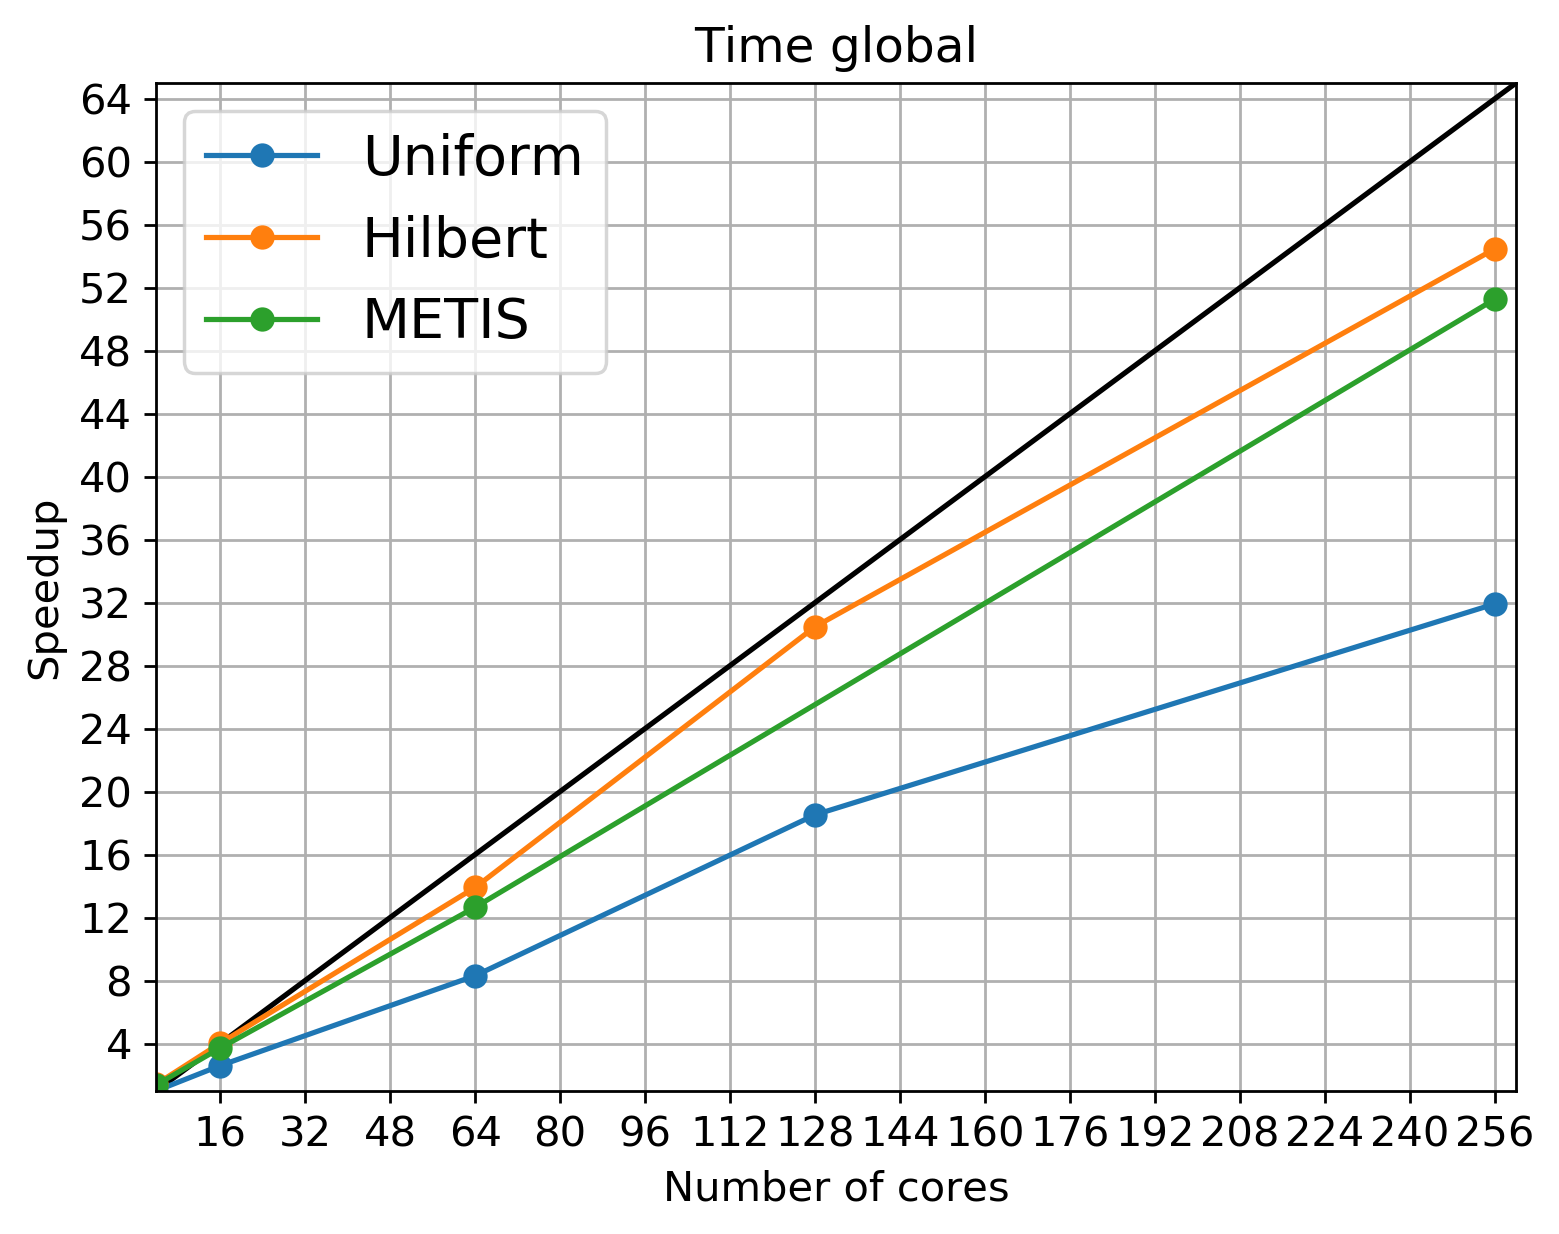
\includegraphics[width=1.0\linewidth]{plot4_upd_global.png}}
    \end{minipage}
    \hfill
    \begin{minipage}[h]{0.48\linewidth}
    \center{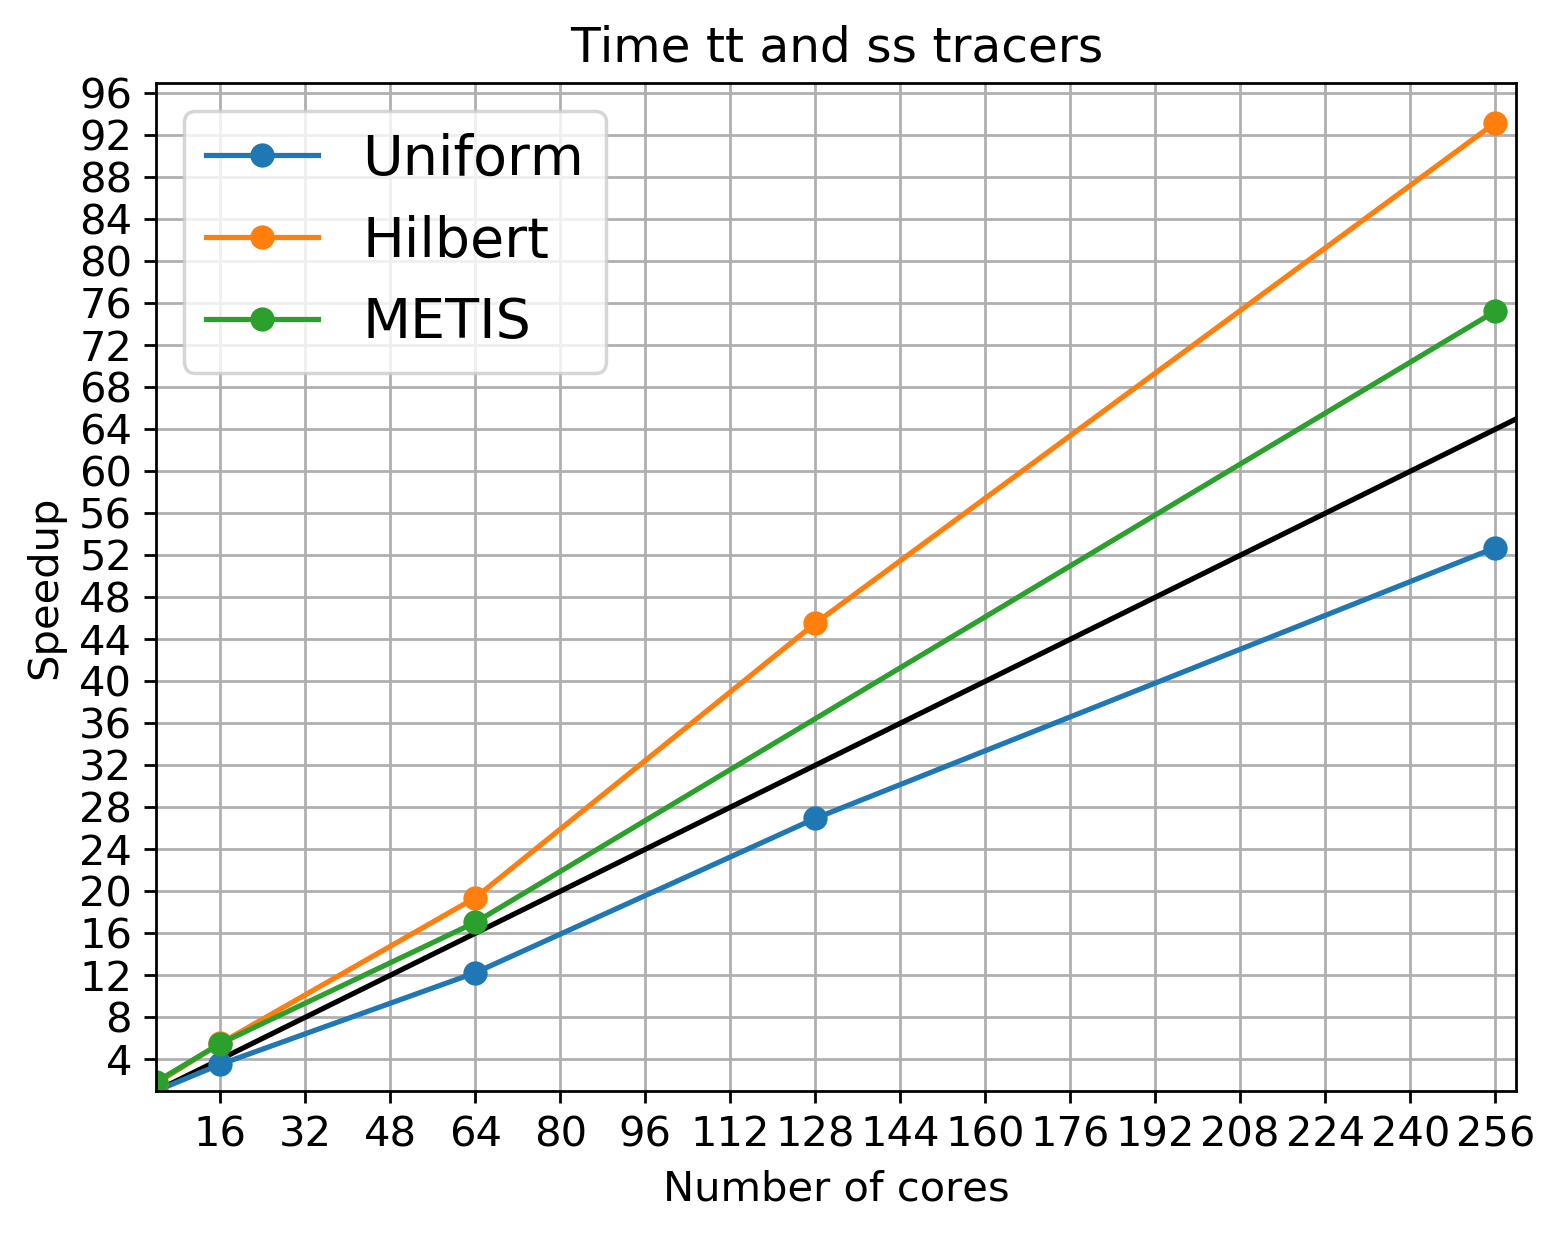
\includegraphics[width=1.0\linewidth]{plot4_upd_tt_ss.png}}
    \end{minipage}
    \caption{Модель океана INMOM. Ускорение метода разбиения с использованием кривых Гильберта в сравнении с равномерным разбиением и с METIS. 1) Общее время работы модели. 2) Расчет температуры и солености. 
    Чёрная линия соответствует линейному ускорению.}
    \label{fig:inmom_hilbert1}
    \end{figure}
    
     \begin{figure}[htb!]
    \begin{minipage}[h]{0.48\linewidth}
    \center{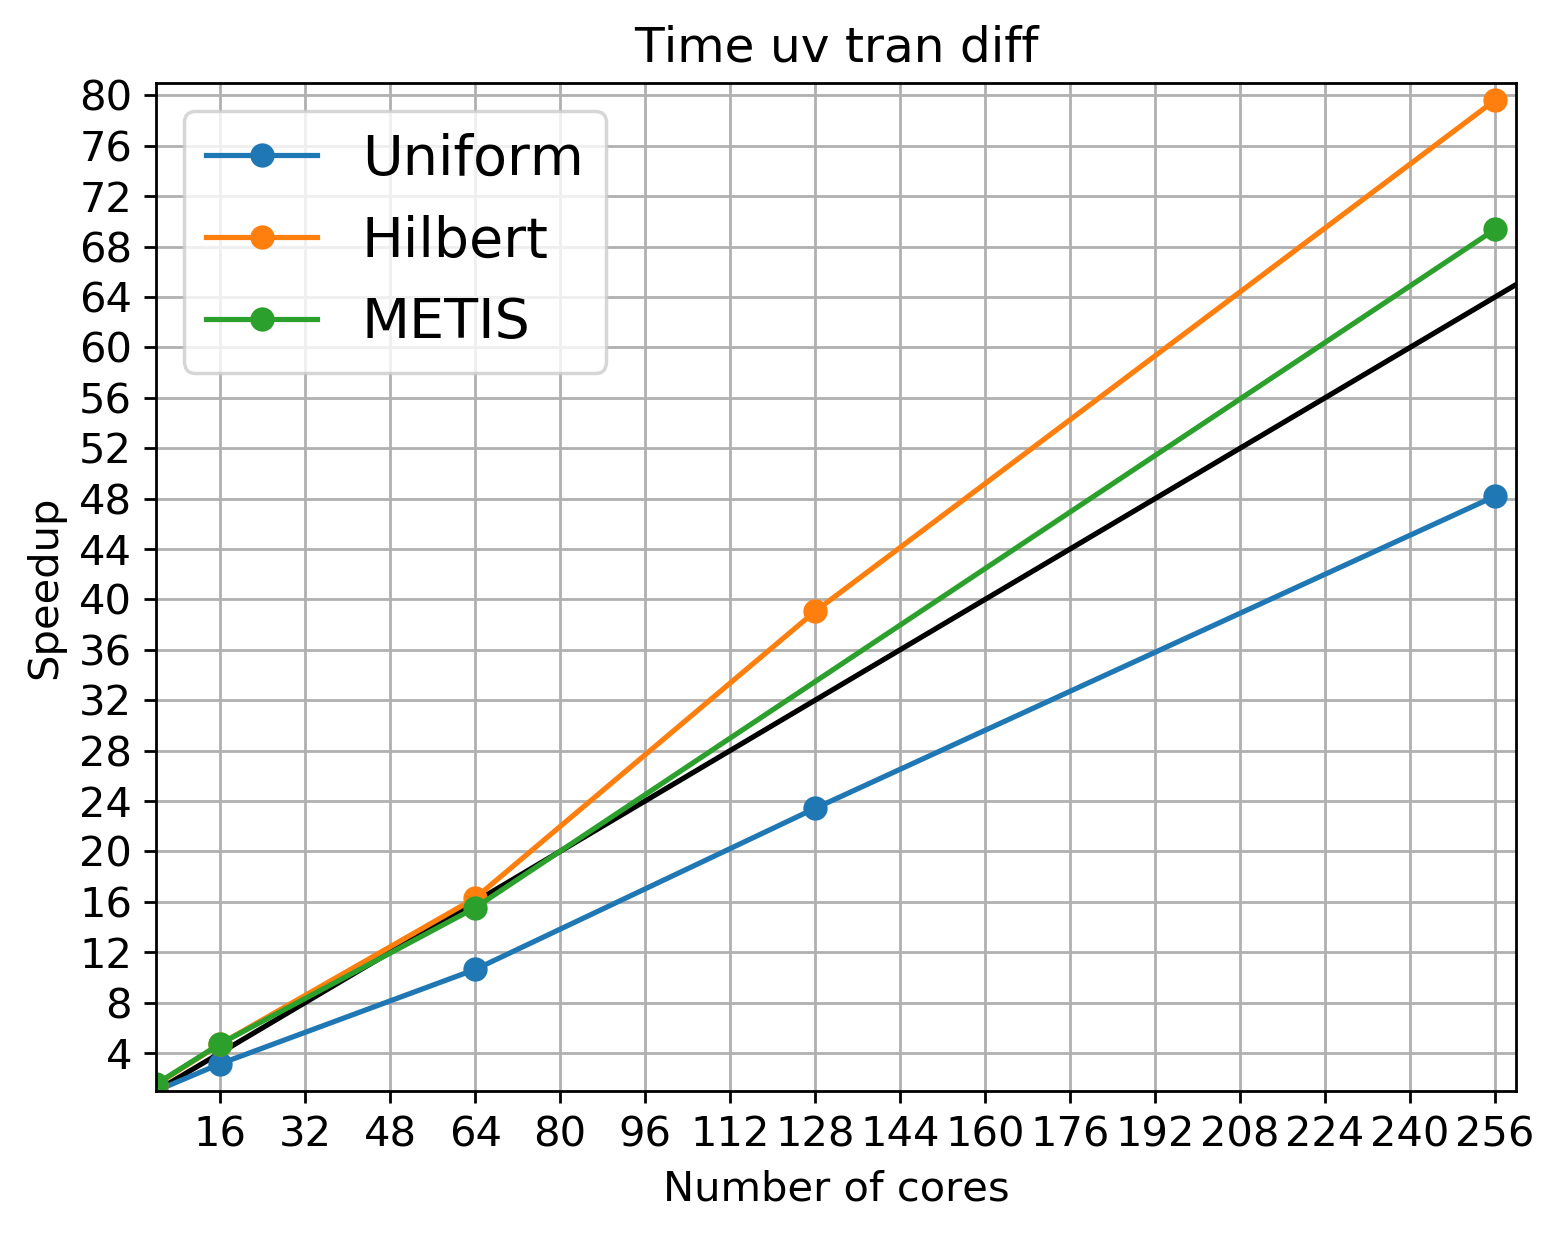
\includegraphics[width=1.0\linewidth]{plot4_upd_uv_tran_diff.png}}
    \end{minipage}
    \hfill
    \begin{minipage}[h]{0.48\linewidth}
    \center{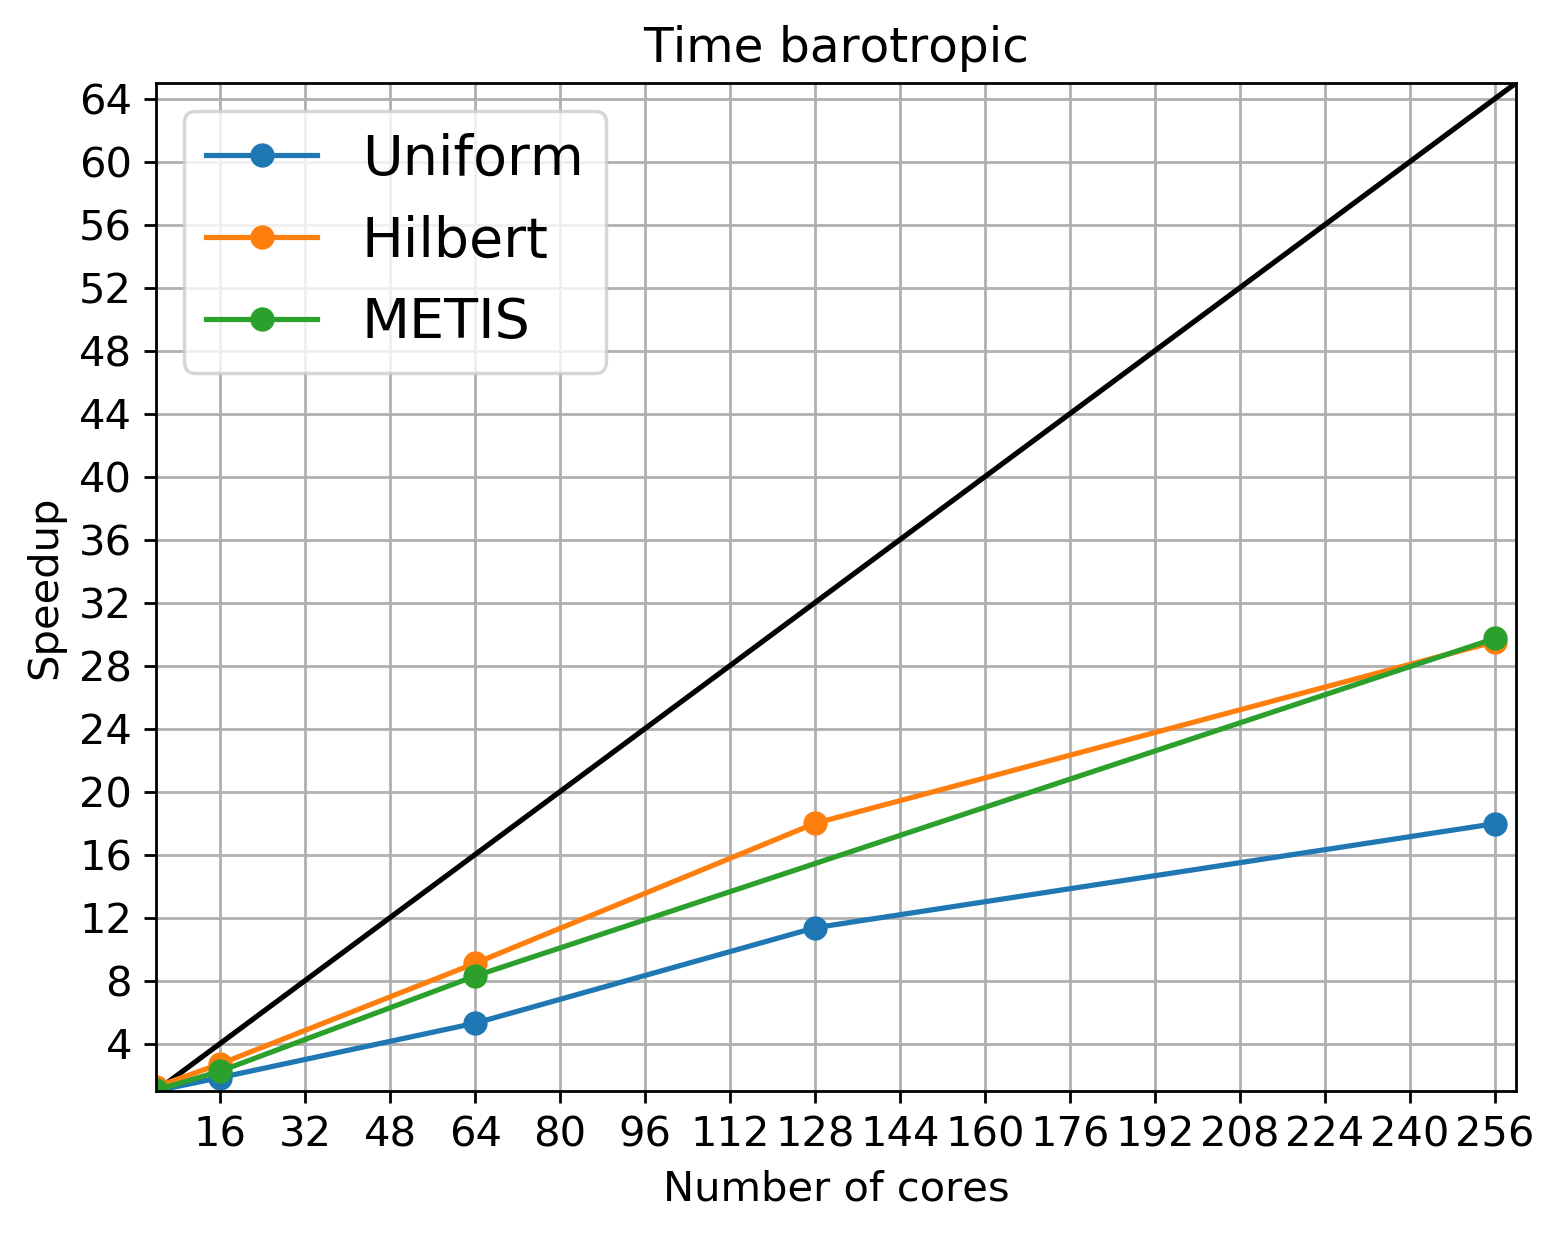
\includegraphics[width=1.0\linewidth]{plot4_upd_barotrop.png}}
    \end{minipage}
    \caption{Модель океана INMOM. Ускорение метода разбиения с использованием кривых Гильберта в сравнении с равномерным разбиением и с METIS. 1) Расчет переноса и диффузии для компонентов скорости. 2) Баротропная адаптация. 
    Чёрная линия соответствует линейному ускорению.}
    \label{fig:inmom_hilbert2}
    \end{figure}


	%В целом, для рассмотренной задачи выяснилось, что можно использовать как балансировку нагрузки с использованием кривых Гильберта так и METIS. 
    Отметим, что метод балансировки с использованием кривых Гильберта строит разбиения в несколько раз быстрее METIS, 
    но для рассматриваемой задачи это незначительно, т.к. расчетное время на порядок больше чем время построения разбиения. 
    Однако, алгоритм балансировки с использованием кривых Гильберта будет давать существенные преимущества по сравнению с METIS, когда задача будет упираться во время построения разбиения, 
    например, на очень большой расчетной области и с адаптивной сеткой.
    Также описанный алгоритм балансировки предпочтительнее чем METIS, так как он реализован непосредственно в модели
    и его реализация довольно простая в отличие от того, что реализовано в METIS.
    METIS - это библиотека для разбиений вообще произвольного вида, в ней реализованы довольно громоздкие методы, основанные на графах.
    А балансировка с использованием кривых Гильберта - это геометрический метод, который сильно проще и очень хорошо подходит именно для рассматриваемой задачи.  
    Используя описанный алгоритм балансировки нагрузки, у сигма-модели океана INMOM не будет привязки к сторонней библиотеке,
    поэтому дальнейшая разработка, поддержка и улучшения этого инструмента будут легче чем работа с METIS.
    
%    \begin{figure}[htb!]
%	\center
%	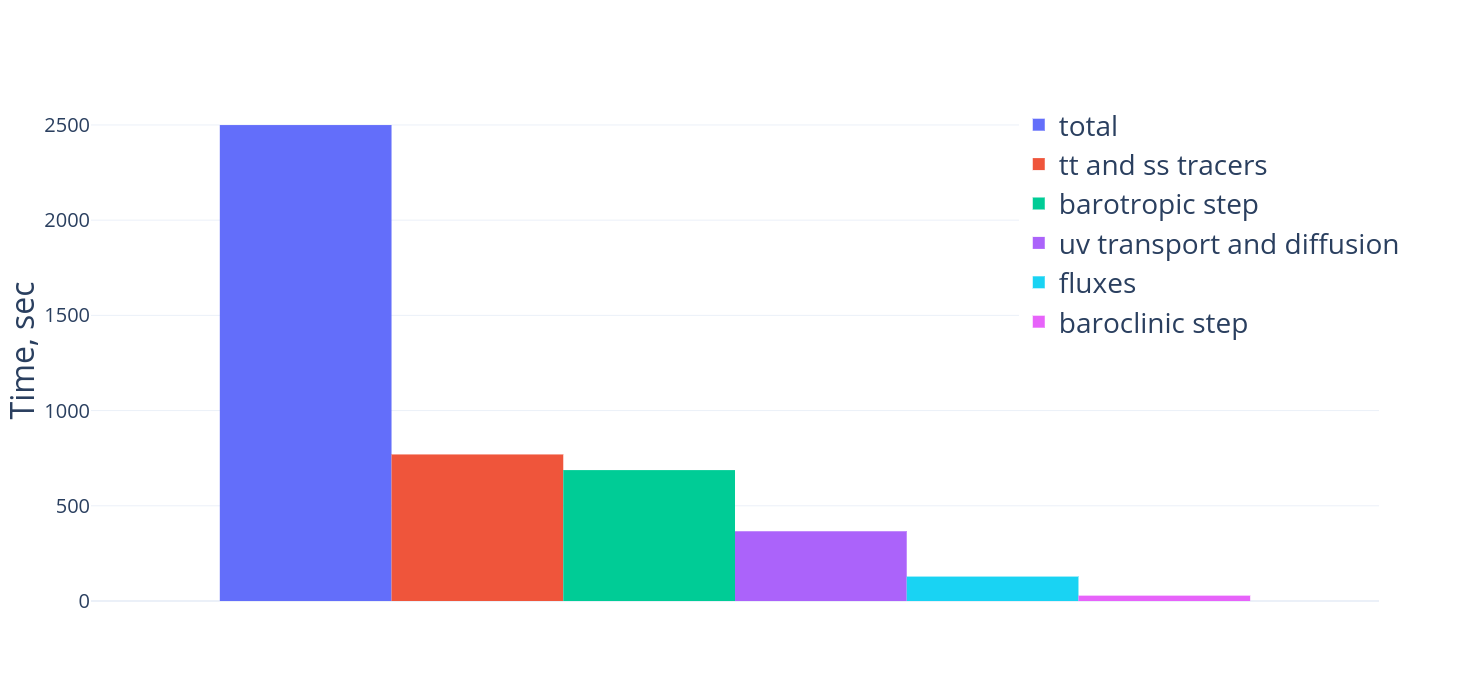
\includegraphics[scale = 0.3]{./data_final/TimeModelSteps.png}
%	\caption{Время работы разных блоков параллельной сигма-модели океана INMOM на 4 ядрах без балансировки нагрузки вычислений. 
%	total - общее время работы модели; 
%	tt and ss tracers - расчет температуры и солености; 
%	barotropic - баротропная адаптация; 
%	uv transport and diffusion - расчет переноса и диффузии для компонентов скорости;
%	fluxes - расчет потоков на поверхности и дне; 
%	baroclinic - бароклинная адаптация.}
%	\label{fig:timemodelsteps}
%	\end{figure}

\FloatBarrier
